\chapter{Implementation}\label{ch:implementation}

%\Todo{Here we can put pictures and codes snippets}\\

%Instead of having a huge amount of different pre-recorded sound files, which need a lot of space, we eliminate the problem to a \colorbox{pink}{2D look up}, where the algorithm matches the object first and then the exact point of the object that collided with some other object.
%

All synthetic sounds have been created in Pd patches and are interpreted by Heavy which generates audio plugins and a C\# interface for Unity. This C\# script is attached to the GameObject in the scene so that the sound is processed within the game world.

We have created our own script that assigns to every one of the objects  the modal parameters we extracted in the analysis part with the ChucK code. This is done independently of synthesis methods used here below.

\section{Impact Sounds}
%\Todo{decribe the patch, describe the sound (starts low, goes to max ampl and then decays etc)}\\
%\Todo{Put spectrogram pictures of the sounds to describe them}
%
\subsection{Sinusoidal Additive Synthesis}

In this section we describe in depth how the Pd patch corresponding to the sinusoidal additive synthesis of impact sounds works. The patch attempts to translate equation \ref{eq:modal_response} into the programming language of Pd. Some of its terms are referenced in the following explanation.

First of all the frequencies and amplitudes matching the ten modes of the object are initialized. We can therefore feed these frequencies, which we identified as $f_n$ in the equation \ref{eq:modal_response}, into the different oscillators. In Pd, oscillators output a cosine wave which is equivalent to $cos(2 \pi f_nt)$ from the equation which suits our purpose perfectly.

We also translate into Pd the expression $e^{-d_n t}$ which corresponds to the damping of every mode $n$. Gaver \cite{gaver1993we} states that for each partial the decay rates $d_n$ are controllable through a parameter $D$ which corresponds to a material and that a useful heuristic, that we use in our patch, is to have $d_n = 2 \pi f_nD$. By experimenting we established that values of $D$ range from approximately 0.0002 for metal to about 0.05 for plastic sounds, with glass, ceramic and wood sounds in between. The higher the damping the higher the values. Then we multiply the damping by the partial's initial amplitude $A_n$ to obtain an amplitude envelope that varies over time and which we multiply by the oscillator's signal. The output is what we call a partial which is illustrated in figure \ref{fig:dampedsignal}. 

\begin{figure}[H]
  \centering
    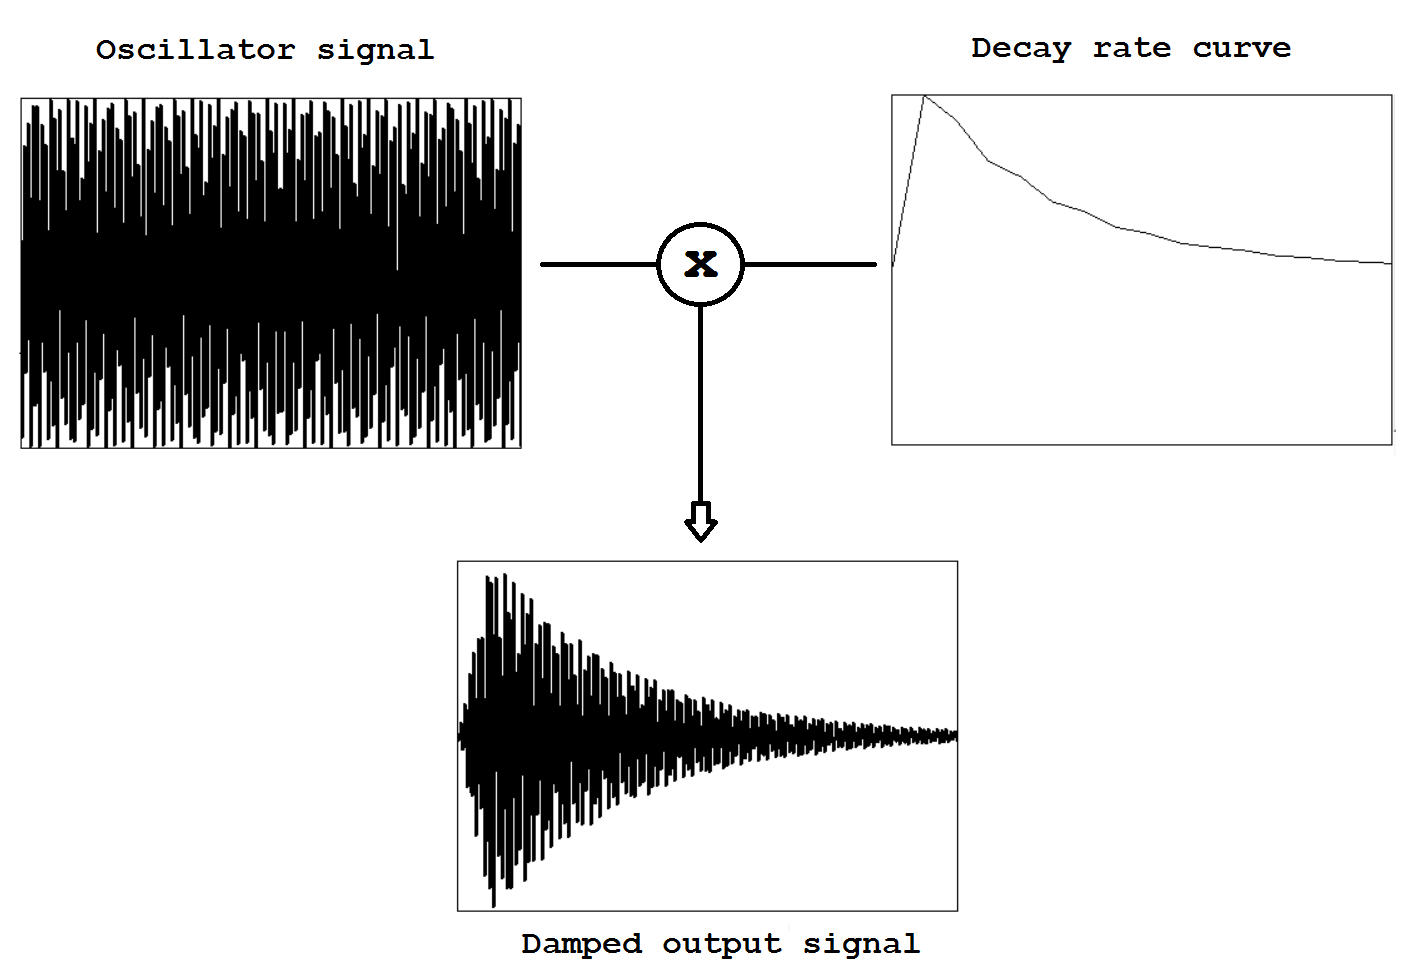
\includegraphics[width=0.7\textwidth]{dampedsignal.png}
      \caption{Diagram showing how the output partial is created from a 5000 Hz cosine wave and a decay rate curve with D = 0.005.}
      \label{fig:dampedsignal}
\end{figure}

The final sound is produced by adding together the ten partials. The resulting signal is multiplied by the magnitude of the impact. \colorbox{pink}{For this we calculate the kinetic energy with Unity's physics components}. As described in \cite{farnell2010designing}, before sending the signal to the DAC we pass it through a clipper that gives richer harmonics and produces brighter sounds the stronger the impact is.

The patch produces an impact sound whenever the OnCollisionEnter() method from Unity is called. This is done when the collider that has the script attached to it touches another collider. When this happens we set the magnitude of the collision and then send an event to excite the patch. This is done by setting the value of $t$ in \ref{eq:modal_response} to zero which increases over time making the sound decay.

\subsection{Filter-based Modal Synthesis}

This synthesis method is based on the utilization of a bank of ten bandpass filters. Pd's bandpass filters have three control inputs as seen in figure \ref{fig:pdbandpass}. The left inlet is the incoming audio signal, the middle one sets the center frequency and the right input sets the Q factor value. The characteristics of these filters define the virtual object.

\begin{figure}[H]
  \centering
    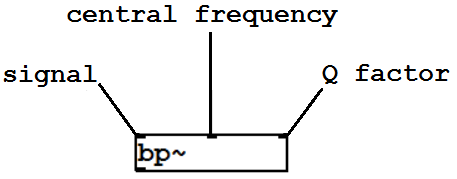
\includegraphics[width=0.5\textwidth]{bandpassfilter.png}
      \caption{Pd's bandpass filter with its three inlets}
      \label{fig:pdbandpass}
\end{figure} 

The same way we did in the previous method, we initialize all ten frequencies and amplitudes of the object. Every frequency $f_n$ is sent into a bandpass filter as the center frequency. 

Every filter is characterized by its Q factor which is directly related to the damping. The higher the value of Q, the narrower the bandwidth and the less the resonator becomes damped. Thus, Q determines the material of the impacted object \cite{gaver1993we}. By manipulating Q we can obtain different material sounds. Through experimentation we have found values of Q that range from about 20 for plastic to 5000 for metal. 

To cause the object to sound we use a short impulse signal that excites the filter. The amplitude of the signal goes from 1 to 0 in 2 milliseconds as represented in figure \ref{fig:impulse}. This impulse is multiplied by the value of the kinetic energy when the object impacts with another. 

\begin{figure}[H]
  \centering
    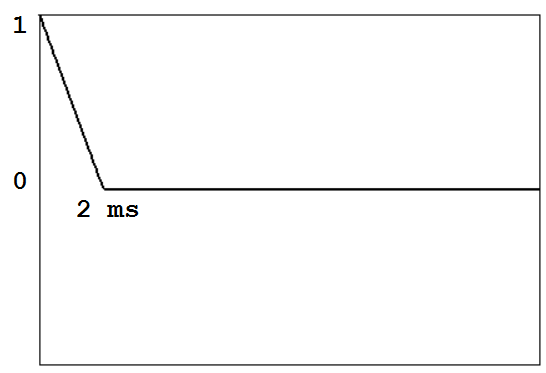
\includegraphics[width=0.5\textwidth]{impulse.png}
      \caption{Impulse signal used to excite the bandpass filter.}
      \label{fig:impulse}
\end{figure} 

The output signal of each of the ten filters is multiplied by the corresponding amplitude $A_n$ of the mode. All ten resulting signals are added together. The signal is sent through a clipper as we did in the previous synthesis method.

\section{Scratching Sounds}

The sound produced by an object that is scraped across a rough surface can be assimilated to a succession of multiple impacts in a short time according to \cite{gaver1993we}. Additionally, the aforementioned paper shows that the resonant modes present in the spectrum of a struck object, are the same as when the object is scrapped. We can then use the same modal parameters as in the impact methods described here above.

\cite{gaver1993we} and \cite{van2001foleyautomatic} propose the use of filters to produce scraping sounds. We therefore choose the filter-based modal synthesis method to model the resonator as seen in the previous section. The difference lies in the signal that excites the model. We implement this by generating a noise impulse waveform that passes through the bandpass filters (put figure and explain how this signal is created, depends on velocity and Q). 

The authors state that the center frequencies of the filters are scaled with respect to the contact velocity. The higher the velocity, the more the proportion of high-frequency energy increases. 


\section{Rolling Sounds}

\section{User Interface}
Here we will describe the \textit{user interface (UI)} of the tool, where sound designers are able to choose the sound they prefer for every object.

The UI is made inside Unity\textregistered, by programming a custom inspector. \textit{Inspector} in Unity\textregistered is a window that shows up after selecting an object, a file etc inside the platform and it displays all information relevant to it.

We also used a custom \textit{GUISkin}, which is a set of settings about the Graphical User Interface (GUI). 
%\begin{figure}[H]
%  \centering
%    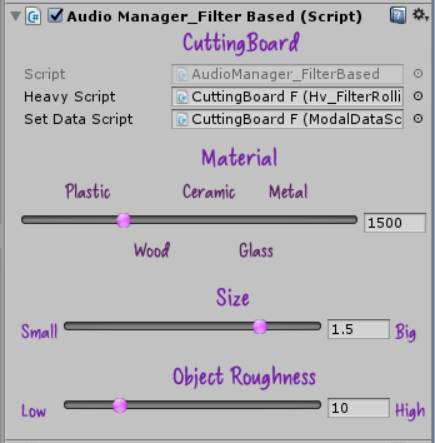
\includegraphics[width=0.5\textwidth]{audio_managerF_inspector.PNG}
%      \caption{The custom inspector inside Unity platform.}
%      \label{fig:custom_insp}
%\end{figure}

\begin{figure}[H]
    \centering
    \begin{subfigure}[b]{0.4\textwidth}
        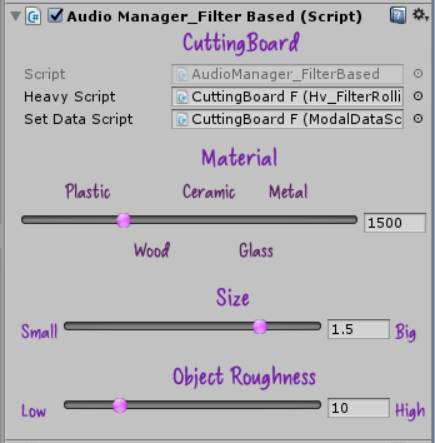
\includegraphics[width=\textwidth]{audio_managerF_inspector.PNG}
        \caption{Filter Based}
        \label{fig:FB}
    \end{subfigure}
    ~ %add desired spacing between images, e. g. ~, \quad, \qquad, \hfill etc. 
      %(or a blank line to force the subfigure onto a new line)
    \begin{subfigure}[b]{0.4\textwidth}
        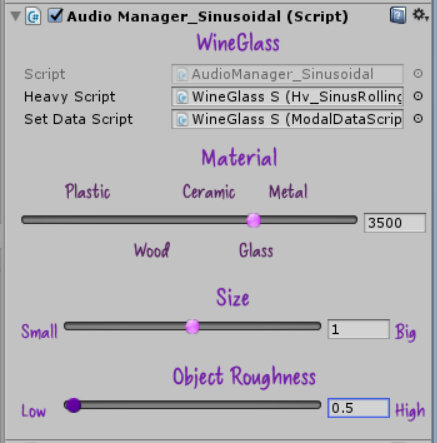
\includegraphics[width=\textwidth]{audio_managerS_inspector.PNG}
        \caption{Sinusoidal}
        \label{fig:sin}
    \end{subfigure}
    \caption{The custom inspector inside Unity platform.}\label{fig:custom_insp}
\end{figure}

When the designer wants to assign the procedural audio component on a Unity game object, he only has to select this game object and then from the Unity menu bar he can select one of the two available methods described above, as seen in figure \ref{fig:menu_item}.
\begin{figure}[H]
  \centering
    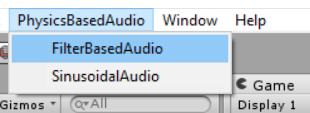
\includegraphics[width=0.5\textwidth]{menuItem.png}
      \caption{Designer can assign the audio manager from the menu bar.}
      \label{fig:menu_item}
\end{figure}

Since every sound is produced from a corresponding real world object, the tool is restricted to the objects available up to this time. Therefore, the designer has to assign a \textbf{``tag''} of one of the eleven objects available on the tool (cooking pot, cup, cutting board, hug, mortar, bowl, plate, rolling pin, wine bottle, wine glass or wok). However, it is easy for her to contribute with new objects to the tool, by following the guide on appendix \ref{ap:guide}.

\subsection{Assignment of Different Materials}
Different materials can be assigned to the objects made for this thesis. The designer is able to choose between \textit{plastic, wood, ceramic, glass and metal} by adjusting the corresponding slider on the interface (see figure \ref{fig:custom_insp}). 

Metallic or glass sounds are more ``ringy'' than wooden or plastic ones that are more ``thud''. We achieve those sounds by changing the \textbf{Q-factor} of the \textbf{band-pass filters} used in the pd patch. Q-factor indicates the power loss in the filter. The higher the Q the less power is lost, so the resonator vibrates longer \cite{bib:Q}.

Using trial and error method, we came out with an average value of the Q-factor for each material and we use it as the default value on the tool. Those values are shown in the table \ref{tab:default_Q}.

\begin{table}[H]
	\centering
    \begin{tabular}{ | l | c | p{5cm} |}
    \hline
    \textbf{Material} & \textbf{Average Q-factor} \\ \hline
    Plastic & 1000 \\ \hline
    Wood & 1500 \\ \hline
    Ceramic & 3000 \\ \hline
    Glass & 3500 \\ \hline
    Metal & 4000 \\
    \hline
    \end{tabular}
    \caption{Default values of Q-factor for each material in the tool.}
    \label{tab:default_Q}
\end{table} 

\subsection{Changing the Size}
In an application, the same object can appear in different sizes, so this thesis takes this into account. It is known that under the same excitation, the smaller the size of an object, the more high-pitched sounds it will produce, because the sound waves travel a smaller distance. Hence, we implemented a slider for the designer to choose the best sound that corresponds to the size of her object. We should note that the middle position of the slider (\textit{size:1}) corresponds to the real object used for the data extraction.

\subsection{Changing the Object Roughness}
Another setting that sound designer is able to tweak is the object roughness. Even though our tool covers several different object materials, not every material has a uniform surface roughness when used in different objects. Adjusting a slider, the designer is able to choose a unique sound for every object of the same material. 


\section{still thinking of the title and placement of this section}
\subsection{Scaling}
As mentioned above, impact sound gets more high-pitched when an object is scaled down and vice versa. To achieve a realistic scaling when the designer uses the build-in scaling feature of Unity\textregistered, the tool calculates the size of the game object on start. More specifically, a \textit{scaling average} is calculated, taking into account all three dimensions (equation \ref{eq:avg_scale}.

\begin{equation}\label{eq:avg_scale}
avgScale = (transform.localScale.x + transform.localScale.y + transform.localScale.z) / 3;
\end{equation}

$avgScale$ is used as an adder to the \textit{size parameter} described above. To avoid distortion in sound and to stay within the audible sound frequencies, we set a limit of adding $8.5$, a number found heuristically. We consider this to be a good choice because Unity uses \textit{meter} as the default unit and since we are mainly focusing on everyday objects, we find it rare for someone to use objects more than $8.5$ times its original size.

Then, the tool checks whether a scale-up or a scale-down was executed. In the first case, we perform a normalization to $1/10$th of the average scale value and we add it to the pitch multiplier \Todo{reference the description of the pitch multiplier}. We apply it to the size slider value and then to the pitch multiplier which we use to re-set the modal frequencies. To be more precise, instead of applying the actual pitch multiplier added with the average scaling, we subtracted from 2 and then we use it ($2-temp$ on the code below). This happens because we reversed the size slider. More specifically, the multiplier directly applied to the frequencies, increases them when it is bigger and decreases them when it is smaller. However, for convenient reasons, we wanted it to be the bigger the multiplier, the bigger the object and reverse. Since $2$ is the biggest value, we normalized it to be the smallest one.

In the second case, we subtract the value from the pitch multiplier. We do not need to normalize the average scaling value, because it is already between $0$ and $1$. Afterwards, we follow the same procedure as above, with one difference; instead of subtracting the new pitch multiplier from $2$ we add it to $1$. This happens because now the biggest value of the size slider is $1$ -since above this it counts as a scale-up- and we still want the reversed value for the slider, so we subtract the subtracted value, making it a plus ($+$).



\begin{lstlisting}[language=C]
// Scale-up
if (avgScale > 1f)
{
	// Normalization
    avgScale /= 10f;
    // Add to the pitch multiplier
    float temp = SetDataScript.multiplier +avgScale;
    // Apply to the size slider
    HeavyScript.SetFloatParameter(Hv_FilterRolling_AudioLib.Parameter.Size, 2-temp);
    // Apply to the pitch multiplier
    SetDataScript.multiplier = 2-temp;
    // Re-set the modal frequencies
    SetDataScript.SetTheFreqs();
}
// Scale-down
else
{
	// Subtract from the pitch multiplier
    float temp = SetDataScript.multiplier - avgScale;
    // Apply to the size slider
    HeavyScript.SetFloatParameter(Hv_FilterRolling_AudioLib.Parameter.Size, 1 + temp);
    // Apply to the pitch multiplier
    SetDataScript.multiplier = 1+ temp;
    // Re-set the modal frequencies
    SetDataScript.SetTheFreqs();
}
\end{lstlisting}



\subsection{OnCollisionEnter}
This is were the tool detects a collision of an object with something else. The collision could be either with the ground, another object from the tool or just an object in the scene.

The first thing that happens when a collision takes place, is to identify what kind of object is the one that collided with something. Hence, a function is called
>>>>>>> 1a362c02b3b7ae0cd6d213f231f01e3ebe707d52



